\documentclass[11pt]{article}
\title{\textbf{Fox-face unit}}
\author{https://github.com/heptagons/meccano/fox-face}
\date{}

\usepackage{../meccano}

\usepackage{tikz}
\usetikzlibrary{calc}

\begin{document}

\maketitle
\begin{abstract}
Fox-face is a group of five meccano strips not forming implicit triangles
but a fox-faced figure used to build a regular pentagon. Here, we'll look for other
angles but not only pentagon's $\cos{2\pi/5}$.
\end{abstract}

\begin{figure}[htb]
\centering
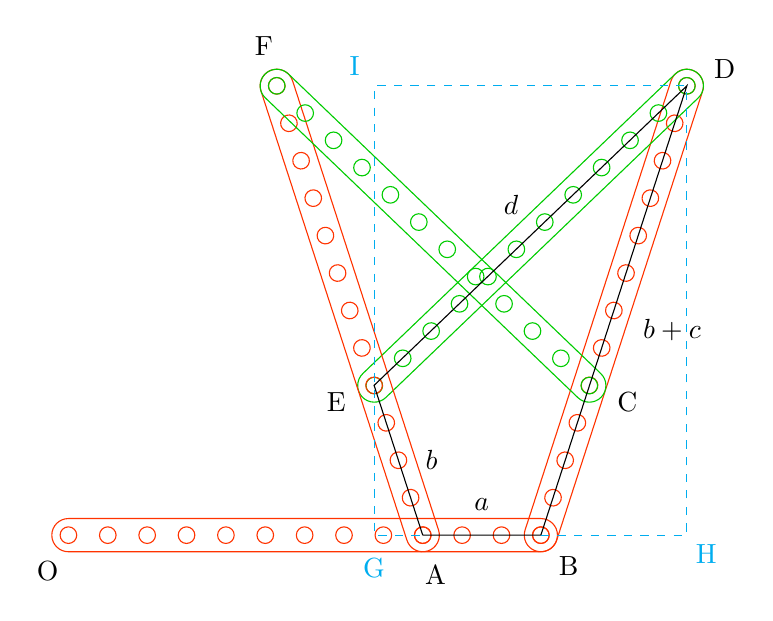
\begin{tikzpicture}

\newcommand{\rod}[4][000000] % [color][n][sep][prop]
{
 \definecolor{main}{HTML}{#1}
 \draw[main] (0,{{2*#4}})
   -- ++({#2*#3},0) arc(+90:-90:{2*#4})
   -- ++({-#2*#3},0) arc(270:90:{2*#4});
 \foreach \x in {0,1,...,#2}
  \draw[main] (\x*#3,0) circle (#4);
}

\def\s {12} \def\f {0.5} \def\p {3pt}
\def\red {FF3300} \def\blue {0000cc} \def\green {00cc00}
\begin{scope}
 \rod[\red]{\s}{\f}{\p} \path (0,0) ++(240:5*\p) node{O};
 \begin{scope}[shift={(\s*\f,0)},rotate=72]
  \rod[\red]{\s}{\f}{\p} \path (0,0) ++(240:5*\p) node{B};
  \begin{scope}[shift={(\s*\f,0)},rotate=180-28.2]
   \rod[\green]{11}{\f}{\p}
   \path (11*\f,0) ++(-20:5*\p) node{E};
  \end{scope}
  \begin{scope}[shift={(\s*\f,0)},rotate=72]
   \path (0,0) ++(240:5*\p) node{D};
  \end{scope}
 \end{scope}
 \begin{scope}[shift={(9*\f,0)},rotate=72+36]
  \rod[\red]{\s}{\f}{\p}
  \path (0,0) ++(-180:5*\p) node{A};
  \path (\s*\f,0) ++(0:5*\p) node{F};
  \begin{scope}[shift={(\s*\f,0)},rotate=180+28.2]
   \rod[\green]{11}{\f}{\p}
   \path (11*\f,0) ++(20:5*\p) node{C};
  \end{scope}
 \end{scope}

\end{scope}

\pgfmathsetmacro{\cosA}{cos(72)}
\pgfmathsetmacro{\sinA}{sin(72)}

\def\a{12*\f}
\def\c{4*\f}
\def\ab{9*\f} % a - b
\coordinate (F) at (\ab,0);
\coordinate (B) at (\a,0);
\coordinate (L) at (\a  + \a*\cosA, 0);
\coordinate (C) at (\a  + \a*\cosA, \a*\sinA);
\coordinate (K) at (\ab - \c*\cosA, \a*\sinA);
\coordinate (I) at (\ab - \c*\cosA, \c*\sinA);
\coordinate (J) at (\ab - \c*\cosA, 0);
\draw[black] (F) 
-- (B) node [midway,shift={(0,1.1em)}]{$a$}
-- (C) node [midway,shift={(+2.1em,-.7em)}]{$b+c$}
-- (I) node [midway,shift={(-.7em,1.1em)}]{$d$}
-- (F) node [midway,shift={(1.2em,0)}]{$b$};
\draw[dashed,cyan] (B) 
-- (L) node[shift={(.7em,-.7em)}]{H} 
-- (C)
-- (K) node[shift={(-.7em,.7em)}]{I} 
-- (I)
-- (J) node[shift={(0,-1.2em)}]{G}
-- (F);    
\end{tikzpicture}
\caption{Fox-figure}
\label{fig:fox-face}
\end{figure}

Figure \ref{fig:fox-face} show the so called fox-face unit.
Has five strips of three types:
\begin{itemize}
\item Single $\overline{AB}$ of length $a$.
\item Pair \{ $\overline{BD}$, $\overline{AF}$ \} of length $b+c$.
\item Pair \{ $\overline{DE}$, $\overline{CF}$ \} of length $d$.
\end{itemize}
In other words we have four different distances:
\begin{itemize}
\item $a$ distance of segment $\overline{AB}$.
\item $b$ distance of segments $\overline{BC}$ and $\overline{AE}$.
\item $c$ distance of segments $\overline{CD}$ and $\overline{EF}$.
\item $d$ distance of segments $\overline{DE}$ and $\overline{CF}$.
\end{itemize}
We are going to test several values of $(a,b,c,d)$ and calculate the angle $\angle{HBD}$.
First we'll calculate a formula and then we'll run a program iterating integer values.

\section{Algebra}
From figure \ref{fig:fox-face} we define $\theta$ = $\angle{HBD}$ and have cosines and sines:
\begin{align}
\theta &\equiv \angle{HBD} = \angle{GAE}\\
\overline{BH} &= (b+c)\cos{\theta}\\
\overline{DH} &= (b+c)\sin{\theta}\\
\overline{AG} &= b\cos{\theta}\\
\overline{EG} &= b\sin{\theta}
\end{align}
We calculate $d$ in function of $(a,b,c)$:
\begin{align}
d^2 &= (\overline{DE})^2\\
 &= (\overline{DI})^2 + (\overline{EI})^2\\
 &= (\overline{AG} + \overline{AB} + \overline{BH})^2 + (\overline{DH} - \overline{EG})^2\\
 &= (b\cos{\theta} + a + (b+c)\cos{\theta})^2 + ((b+c)\sin{\theta} - b\sin{\theta})^2\\
 &= (a + (2b+c)\cos{\theta})^2 + (c\sin{\theta})^2)\\
 &= a^2 + 2a(2b+c)\cos{\theta} + (2b+c)^2\cos^2{\theta} + c^2\sin^2{\theta}\\
 &= a^2 + 2a(2b+c)\cos{\theta} + (4b^2 + 4bc + c^2)\cos^2{\theta} + c^2\sin^2{\theta}\\
 &= a^2 + 2a(2b+c)\cos{\theta} + (4b^2 + 4bc)\cos^2{\theta} + c^2\\
 &= 4b(b + c)\cos^2{\theta} + 2a(2b+c)\cos{\theta} + a^2 + c^2
\end{align}
Let do $X = \cos^2{\theta}$ so last equation can be written as:
\begin{align}
4b(b + c)X^2 + 2a(2b+c)X + a^2 + c^2 - d^2 &= 0\\
\end{align}
So we can calculate $X = \cos^2{\theta}$ with the quadratic formula:
\begin{align}
\cos{\theta} &= \frac{-2a(2b+c) \pm \sqrt{4a^2(2b+c)^2 - 16b(b+c)(a^2 + c^2 - d^2)}}{8b(b+c)}\\
 &= \frac{-a(2b+c) \pm \sqrt{a^2(2b+c)^2 - 4b(b+c)(a^2 + c^2 - d^2)}}{4b(b+c)}\\
\end{align}

\end{document}

